% Course report using the unchanged ICCP 2026 IEEEtran class and 10pt setting.
% Updated from the 31 October supplementary physical experiment, not pooled
% with the prior five-trial exploratory dataset. No conference submission.
\documentclass[10pt,journal,compsoc]{IEEEtran}
\newif\ifpeerreview\peerreviewfalse
\usepackage[nocompress]{cite}
\usepackage{url}
\usepackage{amsmath,amssymb,graphicx}
\usepackage{needspace}
\title{LiDAR-Guided Reconstruction of Axial Motion Blur with Coded Monitor Illumination}
\author{Jarvis Du, Qi Wang, Sai S. Vissavajjhala, and Marco Pham%
\IEEEcompsocitemizethanks{\IEEEcompsocthanksitem MECH5720 Major Project 2026, School of Aerospace, Mechanical and Mechatronic Engineering, The University of Sydney.}}
\begin{document}
\IEEEtitleabstractindextext{%
\begin{abstract}
We built a camera system to study blur as a printed target moves toward the camera during one exposure. A fixed depth sensor records the hand push, and a monitor changes the illumination. Twelve independent pushes cover steady and coded light under two motion instructions. Our main comparison uses six coded exposures and changes only the depth history assumed in reconstruction. Measured depth improves peak signal-to-noise ratio by a mean of 3.04 decibels over a straight-line depth estimate, with a sample standard deviation of 3.67 decibels. Five of six trials improve, and the mean structural-similarity gain is 0.084. Five trials also beat the blurred input, with a different trial failing that comparison. Stationary controls, timing fits and sensitivity checks support a conditional benefit from measured motion. The experiment uses reference-assisted reconstruction, with optical timing, target pose and focus still limiting recovery.
\end{abstract}
\begin{IEEEkeywords}
Axial motion, LiDAR, coded illumination, image reconstruction, experimental characterization.
\end{IEEEkeywords}}
\maketitle
\raggedbottom
\section{Introduction}
A target moving toward a camera grows in the image during exposure. Different image points blur by different amounts, so a single translation-invariant convolution generally cannot describe the blur. A hand push also varies in speed. Measuring depth during exposure could give a better estimate of this changing magnification, while coded illumination changes the contribution of each target position to the photograph.

We ask whether measured depth improves reconstruction of the same coded image compared with a straight line between the same exposure-endpoint depths. The comparison holds the image, illumination history, endpoint geometry, solver and scoring region fixed. We also compare each reconstruction with the blurred input to check whether a better motion estimate actually improves the image.

We built a manual guide path and used an existing upright target stand. The camera, depth board and mounting plate came from the lab kit. Monitor illumination and concurrent image, depth and command logs let us model motion within a conventional long exposure. Our processing aligns these records, constructs a scale-blur operator and estimates the sharp image. All motion was produced by hand. This report presents the supplementary physical dataset and every primary outcome; the earlier five-trial pilot used a different protocol and is kept separate.

\section{Literature Review}
Raskar et al.\ applied temporal coding using a fluttered shutter to encode motion within the exposure and deblur images\cite{raskar}. We draw inspiration for the use of temporal coding, implementing the method using illumination and modeling axial scaling of the image. Our binary pattern is not optimized and is quite short. Their lateral-motion results are motivating to conduct the experiment, but do not constitute a demonstration that coding will benefit this apparatus.

We apply a total variation (TV) regularization to keep noise down, while still preserving edges\cite{rof}. The solver is an accelerated proximal-gradient algorithm based on FISTA\cite{fista}. It involves an approximate TV proximal step, for which we check numerical stability. Endpoint registration is based on scale-invariant features\cite{lowe}. Pixel error is measured with peak signal-to-noise ratio (PSNR), and the quality of local structure is measured by structural similarity (SSIM)\cite{ssim}. The inclusion of the blurred input image as a baseline provides a check of whether the resulting reconstruction helps to make a better photo in addition to the assumed motion model.

\section{Method and Experimental Apparatus}
\subsection{Physical implementation}
The OV5647 camera, Raspberry Pi 3 B+ and LightRanger 14 Click (TMF8829) are fixed on a tripod. We retained the Lab~1 kit lens, with nominal focal length approximately 30\,mm. Tape holds the depth board above the camera, leaving its optical window clear. Two team-built guide edges constrain a sliding base carrying a printed USAF target in an existing upright stand (Fig.~\ref{fig:apparatus}). An ASUS ROG Strix XG27UCGR monitor (27-inch, native $3840\times2160$) illuminates the paper from the side. We checked that the selected depth zones saw the paper: placing the monitor in the ranging field had previously caused foreground returns.

\begin{figure*}[t]
\centering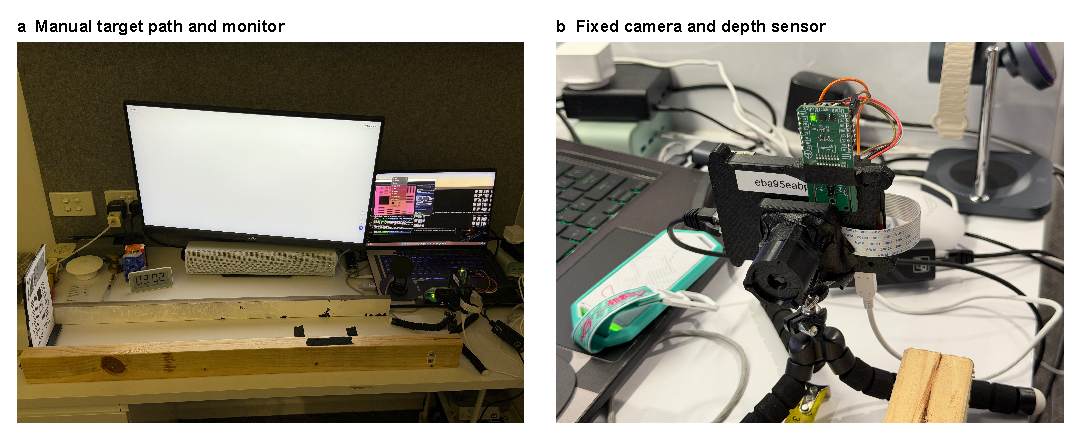
\includegraphics[width=\textwidth]{images/apparatus.pdf}
\caption{Apparatus used for the supplementary experiment. (a) Printed target, manual guide path, side monitor and fixed sensors. (b) Camera and depth board on the kit plate. The team built the guide; the upright target stand and kit plate were supplied. The photographs show placement; alignment and mounting stiffness were not measured.}
\label{fig:apparatus}
\end{figure*}

The base front moves from 75 to 65\,cm toward the camera. The paper lies 22\,mm behind it, giving $D_{\rm paper}=D_{\rm edge}+22$\,mm. This converts the position reference; it does not measure sensor bias because the ruler zero was not surveyed against the optical origin. We kept focus, aperture, monitor position and brightness fixed. The monitor was set to 160\,Hz and brightness-menu value 90; optical transition times and luminance were not measured independently.

\Needspace{10\baselineskip}
\subsection{Acquisition and independent repeats}
The dataset contains 40 runs and 1239 readable DNG images, covering calibration, stationary controls and 16 motion attempts. Twelve eligible independent pushes cover coded/steady-white illumination and smooth/variable push instructions, with three pushes in each cell. For variable pushes, the operator deliberately changed speed; for smooth pushes, the operator tried to keep the motion steady. Both instructions still allowed measured velocity to vary. We retained two pilots and two weak-motion originals outside the primary set, and collected extra independent pushes to replace the weak variable-motion attempts.

Each run saves repeated camera DNGs and continuous $8\times8$ depth arrays. Coded runs also save received illumination events. We select one exposure per push for the primary analysis, so multiple frames and zones do not count as independent trials. Exposure and analogue gain were requested at 1\,s and 1. Metadata give an exposure of 999942\,$\mu$s; actual gain was not independently checked. Acquisition is $640\times480$, reduced to $240\times180$ linear-green images for analysis.

The monitor repeats \texttt{1101001101} in nominal 200\,ms states, giving a 2\,s period and 60\% white duty cycle. We play the code for 12\,s within a 20\,s recording. The camera integrates throughout each exposure while the monitor changes the paper's illumination. Since one second covers only part of the code period, we use the state history logged for that exposure to calculate its weights. White and coded runs involve separate pushes, with unmatched trajectories and light dose.

\subsection{Exposure selection}
We fixed an exploratory selection rule before computing reconstruction scores, without preregistration. A primary exposure needs depth coverage, reliable event coverage for coded light, an approaching target and at least 15\,mm travel during integration. We reject windows crossing anomalous event intervals, then select the largest travel for smooth pushes or the largest departure from endpoint-linear depth for variable pushes. The two weak originals reach only 9.05 and 6.99\,mm maximum travel and are scored separately. One coded run has an event freeze after the selected window; its earlier covered window remains usable. Event counts alone would not reveal this problem.

\section{Timing and Calibration}
\subsection{Clock convention and measurement density}
We align the logs on the Pi monotonic clock. Its calendar was incorrect during recording, so original folder dates serve only as identifiers. We take the camera exposure window as $[t_s-T,t_s]$, interpreting $t_s$ as the first-row readout/exposure-end timestamp and $T$ as the recorded exposure. Rolling-row timing was not measured. Depth and screen logs use host receipt times; the saved device ticks and player clock were not calibrated to this timebase.

Each selected coded exposure contains 10--11 valid received depth frames in one second. We take the median of the central four zones (rows 4--5, columns 4--5, one-based), requiring at least three positive zones, depth 200--2000\,mm and within-region spread no greater than 50\,mm. We omit the known startup sample and interpolate between received frames. Raw depth is used without subtracting the 22\,mm base-to-paper offset.

\begin{figure*}[t]
\centering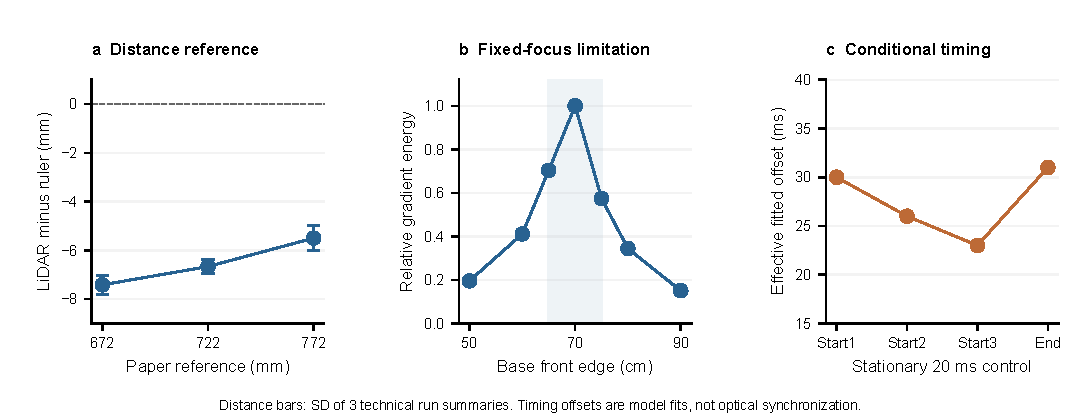
\includegraphics[width=\textwidth]{images/acquisition_bounds.pdf}
\caption{Acquisition checks. (a) Depth residual against the paper reference, including the 22\,mm base-to-paper offset. Bars show sample SDs of three technical run summaries; optical-origin uncertainty remains. (b) Registered gradient energy relative to 70\,cm shows fixed-focus variation. It is a proxy of sharpness but it does not measure the resolution. The range 65--75\,cm base that was kept for use is shaded. (c) Short-exposure controls give fitted offset (effective); the optical synchronization was not measured.}
\label{fig:bounds}
\end{figure*}

\subsection{Stationary checks}
At paper references 672, 722 and 772\,mm, three technical run summaries give depths of $664.58\pm0.38$, $715.33\pm0.29$ and $766.50\pm0.50$\,mm (mean $\pm$ sample SD). The residuals are $-7.42$, $-6.67$ and $-5.50$\,mm. One near-labelled record matches the far position. It is retained as a position/reference discrepancy but excluded from this summary. Given that the origin in the optical data is not defined, the residual cannot be attributed completely to sensor errors.

\Needspace{14\baselineskip}
Stationary 19.969\,ms controls give fitted screen offsets of 30, 26 and 23\,ms initially, and 31\,ms at the end (end-fit $R^2=0.985$). We use 26\,ms as an effective command-to-image offset. Each one-second control has only six covered observations, with weaker transferred-fit agreement ($R^2=0.814$, 0.607, 0.525). The short-exposure fit therefore leaves uncertainty in the long-exposure illumination history. The fixed-patch black/white raw-intensity ratio varies from about 0.167 to 0.211; we use 0.19 in the main model.

Relative gradient energy is 0.70 at 65\,cm and 0.57 at 75\,cm, compared with 70\,cm. It falls to 0.20 and 0.15 at 50 and 90\,cm (Fig.~\ref{fig:bounds}). These fixed-focus checks led us to restrict motion to the narrower range, where some defocus still remains. The selected motion images and final controls are unclipped; two initial white controls each contain one clipped raw pixel. The reference is the median of ten static 100\,ms frames at the nominal 70\,cm base position. These frames form one reference, not ten independent experimental repeats.

\section{Reconstruction and Evaluation}
\subsection{Linear images and empirical axial geometry}
We correct DNG values using per-channel black levels and white level, average the two green samples per Bayer cell, then resize by area averaging. The linear images for inversion are not JPEG-processed and do not apply any display gamma. SIFT feature matches and RANSAC similarity fits relate stationary early/late frames to the sharp reference; selected moving frames are excluded from endpoint fitting. The input and reference are separately globally normalized with the 3rd/97th-percentiles for contrast matching help. All reconstructions use the same input transform.

\Needspace{8\baselineskip}
Endpoint scales calibrate a restricted axial model. With far/near depths $z_f,z_n$, scale ratio $R$, reference depth $z_r$ and a fitted fixed pivot,
\begin{equation}
\beta(z)=\frac{z^{-1}-z_f^{-1}}{z_n^{-1}-z_f^{-1}},\qquad
s(z)=R^{\beta(z)-\beta(z_r)}.
\label{eq:scale}
\end{equation}
This interpolates log scale over inverse depth using the measured endpoints, without requiring an exact optical-origin distance from the ruler. The main dynamic warp scales about the pivot. Endpoint rotation is used for reference registration and enters the dynamic warp only in a sensitivity check. Range alone does not recover continuous target tilt or lateral drift.

\begin{figure}[t]
\centering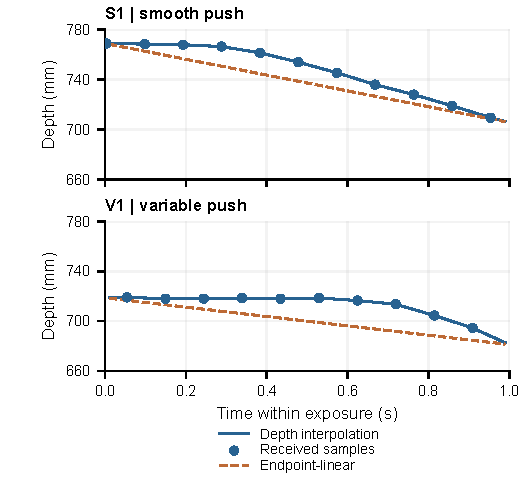
\includegraphics[width=\columnwidth]{images/trajectories.pdf}
\caption{Depth during two selected exposures. S1 and V1 contain 11 and 10 valid received samples. The models share the same exposure-boundary depths and differ only in the interior trajectory. A smooth-push instruction does not impose constant speed.}
\label{fig:depth}
\end{figure}

\Needspace{12\baselineskip}
\subsection{LiDAR-guided axial scale-blur model}
An exposure combines differently scaled views of one sharp reference-plane image $x$. We write the observation $y$ as
\begin{equation}
\begin{aligned}
y&=A(z,u)x+\epsilon,\\
A&=\sum_{k=1}^{48} w_k W[s(z_k)],\\
w_k&=\frac{0.19+0.81u_k}{\sum_j(0.19+0.81u_j)},
\end{aligned}
\label{eq:forward}
\end{equation}
Here, $z_k$ is interpolated depth, $W[s(z_k)]$ scales the image about the fitted pivot, and $u_k$ is the logged binary state after the time shift. We approximate the exposure integral with 48 midpoint bins interpolated from 10--11 received depth frames. $W$ uses sparse bilinear interpolation with replicated boundaries. The weights approximate relative irradiance, with 0.19 as the illumination floor in the black state. Each of the columns of $ A $ is the response to one point in the image - a discrete point spread function (PSF). Expansion moves points farther from the fixed scaling pivot more strongly, so the PSF varies spatially across the image. Reconstruction therefore requires inverting a spatially varying operator.

\subsection{TV-regularised reconstruction}
Once the records and endpoint geometry fix $A$, we estimate the image by non-blind, TV-regularised least squares:
\begin{equation}
\hat x=\arg\min_{0\leq x\leq1}\tfrac12\|Ax-y\|_2^2+\lambda\,\mathrm{TV}(x),
\qquad\lambda=0.002.
\label{eq:inverse}
\end{equation}
The data term fits the recorded blur, while TV limits unstable fluctuations. We use 320 outer iterations of an accelerated proximal-gradient scheme inspired by FISTA\cite{fista}, a power-estimated step size and up to 35 inner TV iterations. The TV step is approximate, and clipping constrains intensities to $[0,1]$. The comparator replaces measured $z(t)$ with constant depth velocity between the same boundary depths. Both methods share the image, light weights, geometry, solver and mask. We also evaluate the blurred input and denoise-only processing ($A=I$). Parameters are shared across trials.

\subsection{Scoring and numerical checks}
We map all 16 attempts into one canonical reference frame and fix a geometry-only intersection mask before scoring (Fig.~\ref{fig:mask}). PSNR uses unit intensity range; Gaussian-window SSIM uses $\sigma=1.5$ and population covariance\cite{ssim}. Methods receive no separate post-reconstruction alignment or contrast fit. The reference is used for registration, normalization and scoring, making this a reference-assisted experiment.

Identity, row-sum and adjoint errors are below $8\times10^{-7}$. Synthetic inversion improves PSNR from 13.99 to 27.15\,dB. Doubling the iterations from 320 to 640 changes PSNR by at most 0.049\,dB; changing the bins from 48 to 96 changes it by at most 0.207\,dB. These checks assess numerical integrity. The physical captures test how well the model describes practice.

\begin{figure}[t]
\centering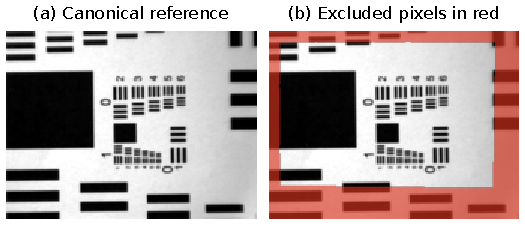
\includegraphics[width=\columnwidth]{images/evaluation_mask.pdf}
\caption{A common reference and common mask for all trials and all methods. Excluded pixels marked in red. Scores use the remaining 28327 pixels (65.6\% of the $240\times180$ image) within the irregular mask, rather than only its boundary or a rectangular display crop.}
\label{fig:mask}
\end{figure}

\section{Results and Analysis}
\subsection{Independent coded pushes}
Table~\ref{tab:six} includes every primary coded push. Targets travel 27.8--63.4\,mm during the selected exposure within the nominal 100\,mm path. The measured trajectories in Fig.~\ref{fig:depth} show motion that the endpoint-linear model misses.

\begin{figure*}[t]
\centering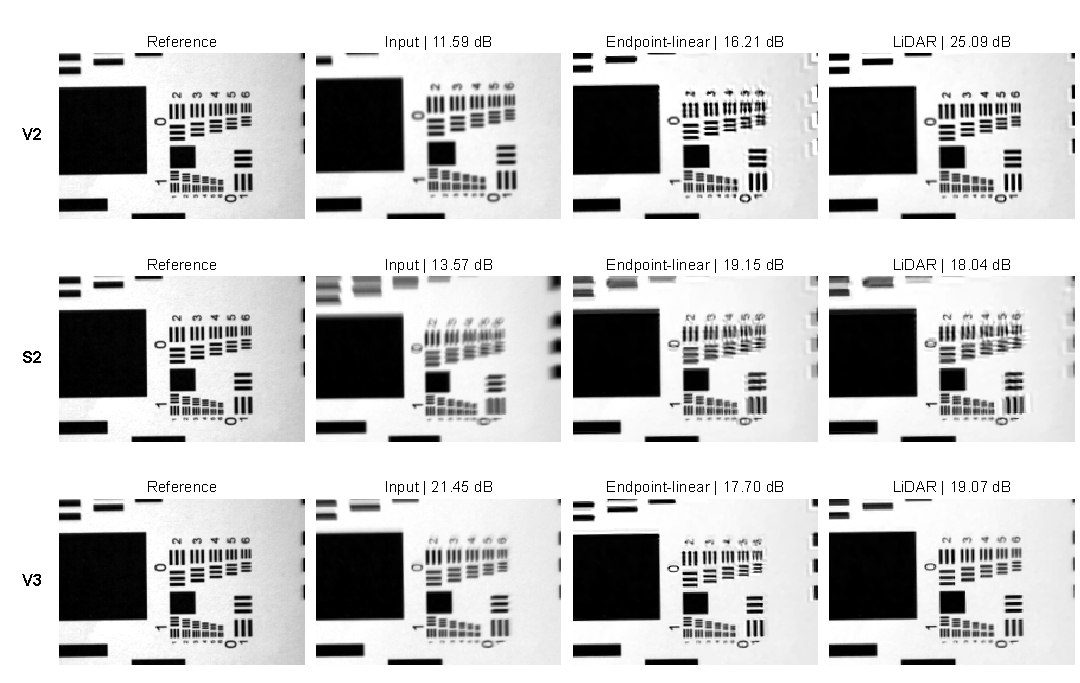
\includegraphics[width=\textwidth]{images/reconstruction_examples.pdf}
\caption{Three outcomes shown with the same canonical crop and linear grayscale range $[0,1]$. V2 has the largest measured-depth advantage; S2 favours endpoint-linear; V3 favours the input over either reconstruction. All six trials appear in Table~\ref{tab:six} and the full analysis gallery. Scoring follows the irregular common mask within each display crop.}
\label{fig:images}
\end{figure*}

\begin{table}[t]
\caption{Six independent coded exposures scored on the common canonical mask. I: blurred input; C: endpoint-linear; L: LiDAR. S/V denote smooth/variable push instructions, with independent repeats numbered 1--3. Actual velocity can vary under either instruction.}
\label{tab:six}\centering
\setlength{\tabcolsep}{3.3pt}\small
\begin{tabular}{lrrr|rrr}\hline
 & \multicolumn{3}{c|}{PSNR (dB)} & \multicolumn{3}{c}{SSIM}\\
Trial & I & C & L & I & C & L\\\hline
S1 & 15.13 & 18.08 & 18.21 & 0.646 & 0.728 & 0.767 \\
S2 & 13.57 & 19.15 & 18.04 & 0.564 & 0.789 & 0.765 \\
S3 & 16.40 & 14.33 & 18.38 & 0.712 & 0.664 & 0.777 \\
V1 & 18.71 & 14.29 & 19.22 & 0.791 & 0.647 & 0.826 \\
V2 & 11.59 & 16.21 & 25.09 & 0.523 & 0.745 & 0.906 \\
V3 & 21.45 & 17.70 & 19.07 & 0.878 & 0.803 & 0.840 \\
\hline\end{tabular}
\end{table}

Measured depth beats endpoint-linear in five of six trials on both metrics. Mean paired differences are $+3.038\pm3.666$\,dB and $+0.0843\pm0.0797$, respectively (sample SD across six independent pushes). Figure~\ref{fig:paired} shows each paired difference and the mean with one sample SD. We report these as descriptive statistics. Against the blurred input, mean gains are $+3.523\pm5.421$\,dB and $+0.1280\pm0.1485$, also with five positive trials. The median paired PSNR gain is 2.706\,dB. Leaving out each push in turn gives mean gains of 1.870--3.869\,dB; omitting V2, the largest gain, gives 1.870\,dB. The primary result retains all six trials; these omissions only check how much each push affects the mean.

\begin{figure}[t]
\centering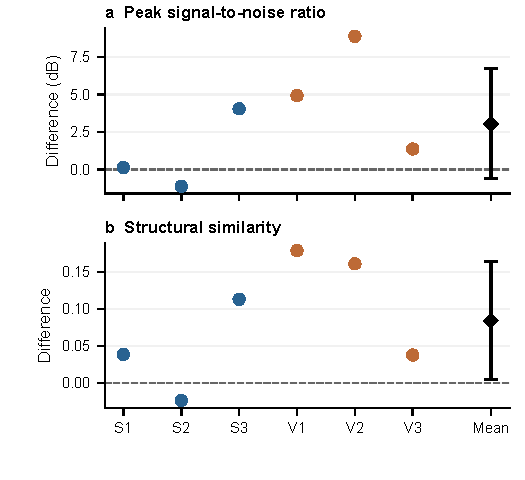
\includegraphics[width=\columnwidth]{images/paired_effects.pdf}
\caption{LiDAR-minus-endpoint-linear differences for all six coded images. The black diamond shows the mean and one sample SD; it is separate from the six trials and does not show a confidence interval. Blue: smooth instructions; orange: variable instructions.}
\label{fig:paired}
\end{figure}

S2 loses 1.115\,dB and 0.0239 SSIM to the endpoint-linear model, although both reconstructions beat its input. V3 improves over endpoint-linear but loses 2.383\,dB and 0.0380 SSIM to input. V2 has the largest paired PSNR gain, 8.880\,dB. Figure~\ref{fig:images} shows V2 and both failure types. These are two different failures: measured depth can lose to the simpler motion model, and motion inversion can degrade an already better input.



\Needspace{24\baselineskip}
\subsection{Examining the failed comparisons}
S2 stays below endpoint-linear across all 13 one-factor settings, with paired PSNR differences from $-1.209$ to $-0.847$\,dB. Changing the tested timing, TV weight, light floor, depth offset or rotation does not reverse that result. This persistence still leaves its physical cause unresolved.

For V3, denoise-only processing gives 21.43\,dB, close to the 21.45\,dB input, while LiDAR inversion gives 19.07\,dB. Most of the loss appears when the motion model is inverted. Increasing the solver from 320 to 640 iterations leaves the score at 19.07\,dB; 96 integration bins give 19.10\,dB. Tested TV weights from 0.0005 to 0.02 give 19.04--19.12\,dB. The loss persists in these checks. Equation~\eqref{eq:forward} fits the recorded blur, so errors in the assumed motion or illumination can lead the solver away from the static reference. Pose, defocus, lighting and timing remain possible contributors; these tests do not separate their effects.

\subsection{Steady-white controls and repeat variation}
Table~\ref{tab:groups} summarizes all 12 primary pushes, with only three independent repeats per cell. The variable-coded cell has a larger mean model advantage than the smooth-coded cell. White-variable reconstruction beats endpoint-linear on average but loses to the input. Motion and integrated illumination differ between the white and coded pushes, preventing a causal comparison of coding.

\begin{table}[t]
\caption{All primary cells, $n=3$ independent pushes each. $\Delta_{LC}$ is LiDAR minus endpoint-linear PSNR (mean $\pm$ sample SD); $\Delta_{LI}$ is LiDAR minus input, also as mean $\pm$ sample SD. Per-trial scores are supplied.}
\label{tab:groups}\centering\footnotesize
\begin{tabular}{llrr}\hline
Light & Instruction & $\Delta_{LC}$ (dB) & $\Delta_{LI}$ (dB)\\\hline
Coded & Smooth & $1.020\pm2.694$ & $3.174\pm1.248$\\
Coded & Variable & $5.057\pm3.758$ & $3.871\pm8.458$\\
White & Smooth & $1.549\pm2.370$ & $3.422\pm2.840$\\
White & Variable & $1.396\pm2.118$ & $-0.932\pm0.898$\\\hline
\end{tabular}
\end{table}

\subsection{Stationary and sensitivity controls}
Relative to denoise-only processing, measured-depth reconstruction gains $3.522\pm5.411$\,dB on average (sample SD, $n=6$), with five trials improving in both metrics. Thus TV denoising alone does not account for the observed mean gain.

Three static depth-driven controls change PSNR by only $+0.001$, $+0.026$ and $+0.010$\,dB relative to input, with SSIM changes $-0.0029$, $-0.0028$ and $-0.0022$. The small changes show how the pipeline behaves without target motion; they provide a control for the moving trials.

\Needspace{14\baselineskip}
Thirteen one-factor checks vary TV weight, light offset, depth timing ($\pm50$\,ms), black-state floor, common depth offset ($\pm22$\,mm) and endpoint rotation. Mean coded LiDAR advantage remains 2.43--3.56\,dB, while individual trial signs can change. This range describes the settings tested separately; it gives neither a statistical uncertainty bound nor a joint worst-case result. Doubling quadrature bins changes the mean advantage from 3.038 to 3.013\,dB. Frozen-geometry replay in a compatible numerical environment changes PSNR by at most 0.0032\,dB, showing that the frozen-geometry calculation is repeatable. Fresh registration can still change subpixel fits.

\section{Limitations and Pitfalls}
Command receipt times and a fitted offset are used to estimate the illumination history. We neither measured optical transitions with a photodetector, nor calibrated the ranging-to-receipt delay or measured the rolling-row skew. The timing perturbations we test represent only some of the possible errors.

We also left out from the scale model continuous tilt and lateral drift, depth-dependent defocus and spatial variation in illumination. We observe a change in sharpness even inside the range retained in our tests of fixed-focus control. The optical origin remains uncertain, and the 22\,mm base-to-paper offset does not provide an independent sensor-bias calibration. These effects are not separated experimentally and we are not able to link either failed comparison to one physical cause.

\Needspace{3\baselineskip}
Reference-assisted registration and contrast normalization limit the scope of the scores. Downsampling and TV may suppress fine bars, and the shared mask depends on reference geometry. Selection was exploratory; all attempts and weak-motion replacements are documented. Six coded pushes and three repeats per cell support descriptive comparisons. Unmatched white/coded motion and light dose prevent a causal claim about coding.

\Needspace{4\baselineskip}
\section{Conclusions and Future Work}
Our manual-push system records long-exposure images alongside depth and monitor-command histories for axial-motion reconstruction. For six independent coded exposures, LiDAR-guided reconstruction gives a mean PSNR improvement of 3.04\,dB over a matched endpoint-linear model. Five trials improve both PSNR and SSIM. S2 lost to that endpoint-linear model, while V3 lost to the blurred input image. The control and numerical verification indicated a conditional gain from measured motion; timing, focus, pose and reference assistance still limit the result.

Given two additional months, we would first measure the optical transition and the rolling row timing, as well as the range origin and the image scale and illumination on the path. Then, we would preregister the selection rules and collect randomized repeated motions, at equivalent light dose. A continuous pose measurement and a defocus model dependent on depth would help disentangle possible causes of failure, before testing the optimal codes.

\section{Reproducibility}
The accompanying package contains the acquisition data, all 16 attempt scores, frozen selections and geometry, source hashes, reconstruction arrays, scripts, dependencies and build instructions. Run \texttt{python reproduce.py} to recalculate saved-array metrics and regenerate the paired-effect and mask figures. Use \texttt{--reconstruct} for all 16 RAW inversions with frozen geometry, or \texttt{--trial S1} for one coded exposure. The README covers the tested environment, hardware records and fresh registration, whose subpixel fits can vary across numerical environments. The earlier five-trial dataset is separate. Public code/data URL: \emph{to be supplied by the authors before submission}.

\begin{thebibliography}{5}
\bibitem{raskar} R. Raskar, A. Agrawal, and J. Tumblin, ``Coded exposure photography: motion deblurring using fluttered shutter,'' \emph{ACM Trans. Graph.}, vol. 25, no. 3, pp. 795--804, 2006, doi: 10.1145/1141911.1141957.
\bibitem{rof} L. I. Rudin, S. Osher, and E. Fatemi, ``Nonlinear total variation based noise removal algorithms,'' \emph{Physica D}, vol. 60, pp. 259--268, 1992, doi: 10.1016/0167-2789(92)90242-F.
\bibitem{fista} A. Beck and M. Teboulle, ``A fast iterative shrinkage-thresholding algorithm for linear inverse problems,'' \emph{SIAM J. Imaging Sci.}, vol. 2, no. 1, pp. 183--202, 2009, doi: 10.1137/080716542.
\bibitem{lowe} D. G. Lowe, ``Distinctive image features from scale-invariant keypoints,'' \emph{Int. J. Comput. Vis.}, vol. 60, no. 2, pp. 91--110, 2004, doi: 10.1023/B:VISI.0000029664.99615.94.
\bibitem{ssim} Z. Wang, A. C. Bovik, H. R. Sheikh, and E. P. Simoncelli, ``Image quality assessment: From error visibility to structural similarity,'' \emph{IEEE Trans. Image Process.}, vol. 13, no. 4, pp. 600--612, 2004, doi: 10.1109/TIP.2003.819861.
\end{thebibliography}

\end{document}
